% STATUS: QUARANTINED. The mechanisms below failed their matched controls.
% See ../METHOD_STATUS.md and ../../METHOD_REDESIGN.md.
\section{方法}
\label{sec:method}

\subsection{问题定义}

设有标注数据集为
\begin{equation}
\mathcal D_l=\{(x_i^l,y_i^l,d_i)\}_{i=1}^{N_l},
\end{equation}
其中 $x_i^l\in\mathbb R^{3\times H\times W}$ 表示田间 RGB 图像，$y_i^l\in\{0,\ldots,C-1\}^{H\times W}$ 表示像素级标注，$d_i\in\{1,\ldots,D\}$ 表示采集域。无标注数据集记为
\begin{equation}
\mathcal D_u=\{(x_j^u,d_j)\}_{j=1}^{N_u}.
\end{equation}
本文考虑背景、麦穗、茎秆和叶片四个类别，即 $C=4$。训练阶段只使用 $D$ 个源域中的有标注和无标注图像，测试目标是直接泛化到未参与训练的目标域 $d^\star$。

本文采用由 Mean Teacher 发展而来的教师--学生框架 \citep{tarvainen2017mean}。学生网络 $f_{\theta_s}$ 接收强扰动图像并通过梯度下降更新，教师网络 $f_{\theta_t}$ 接收弱扰动图像并产生伪标签。教师参数通过学生参数的指数滑动平均更新：
\begin{equation}
\theta_t\leftarrow\alpha\theta_t+(1-\alpha)\theta_s,
\label{eq:ema}
\end{equation}
其中 $\alpha$ 为动量系数。基础分割器由 BEiTv2-Large、ViT-Adapter 和 Mask2Former 构成 \citep{peng2022beitv2,chen2023vitadapter,cheng2022mask2former}。ViT-Adapter 输出四级特征，Mask2Former 使用多尺度像素解码器和掩码查询得到类别概率及掩码概率。本文的结构监督和原型学习均作用于由查询预测组合得到的可微语义概率图。

\subsection{总体框架}

\begin{figure}[!t]
\centering
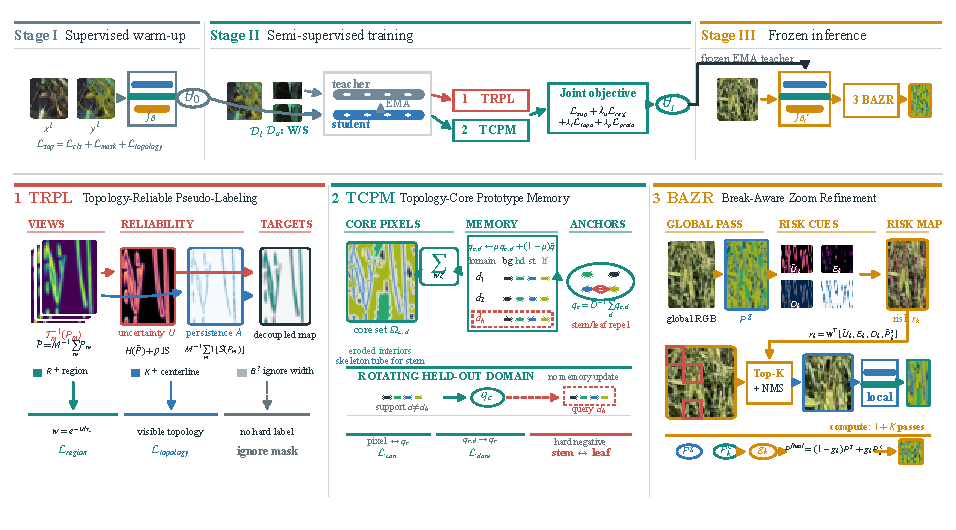
\includegraphics[width=\textwidth]{figures/framework.pdf}
\caption{\METHOD 的三阶段流程与关键算子。上排依次给出监督预热、连续 EMA 教师--学生联合训练和冻结教师推理。下排展开三个创新点：\TRPL 以语义置信度 $Q$ 和双视图分歧 $D$ 形成可靠性 $r$，并用严格骨架共识解耦可靠区域 $R^+$、稳定中心线 $K^+$ 与忽略边界 $B^{?}$；\TCPM 从器官核心 $\Omega_{i,c}$ 分别更新有标注与伪标注类别--域记忆，按样本排除自身采集域后形成类别锚点 $\bar q_c^{(-d_i)}$，再校正可靠区域中偏离该锚点的困难查询；\BAZR 将熵、异常端点、尺度分歧和茎秆先验组合为窗口风险 $r_k$，经 Top-$K$/NMS、局部前向和门控融合得到最终预测。RGB、标注、窗口与裁剪均来自严格对齐的真实样本；底排的概率、可靠性及风险热图依据同一标注几何确定性构造，仅解释空间对齐与运算关系，不表示实验预测。}
\label{fig:framework}
\end{figure}

监督预热、拓扑感知半监督学习与断裂感知推理构成一条连续的信息链（\cref{fig:framework}）。有标注样本首先确定器官语义和茎秆拓扑的共同表征起点 $\theta_0$，教师与学生均由该权重初始化；进入半监督阶段后，教师从第一步起连续执行 EMA，而不再经历冻结后由学生硬覆盖的参数跳变。\TRPL 随后利用无标注图像扩展外观覆盖，将区域可信度与中心线稳定性解耦；\TCPM 把结构可靠核心压缩为跨域类别参照，并将监督传递给同类可靠区域中的困难位置。两条支路共享同一学生特征并通过联合目标相互约束，训练收敛后仅保留 EMA 教师参数 $\theta_t^*$。部署时不再维护学生和原型记忆；\BAZR 从该教师的一次全局前向中评估结构失效风险，把额外计算集中到少量候选窗口。

\subsection{拓扑可靠伪标签学习}
\label{sec:trpl}

\TRPL 借鉴弱到强一致性学习利用教师预测监督强扰动视图的基本形式 \citep{yang2023unimatch}，也保留了 U2PL 和 ST++ 所强调的伪标签可靠性控制 \citep{wang2022u2pl,yang2022stpp}。这些方法把可靠性定义在像素、区域或整幅图像层面，置信度不足的茎秆像素通常被统一丢弃。对小麦图像而言，低置信度并不总意味着器官位置错误：由混合像素和下采样引起的不确定性往往集中在茎秆两侧，而中心位置在不同视图中仍然稳定。soft-clDice 提供了可微的中心线一致性约束 \citep{shit2021cldice}，但它假设监督掩码本身具有可信拓扑，直接用于噪声伪标签可能把偶然误连固化下来。\TRPL 的改动在于先通过多视图一致性确定可见中心线是否可信，再分别处理中心线、区域和边界，而不是对整张伪掩码使用同一阈值或同一拓扑约束。

\subsubsection{双视图可靠性估计}

多组类别阈值与不确定性温度会使伪标签机制难以归因。本文只对无标注图像 $x^u$ 构造原尺度和缩放尺度两个弱视图。第 $m$ 个视图经尺度变换后，其对齐到原图坐标的教师预测为
\begin{equation}
P_m=\mathcal T_m^{-1}
\left(f_{\theta_t}(\mathcal T_m(x^u))\right).
\end{equation}
平均预测 $\bar P=M^{-1}\sum_{m=1}^{M}P_m$ 用于生成类别伪标签 $\hat y(p)=\arg\max_c\bar P_c(p)$。视图分歧采用无需额外温度或权重的总变差距离：
\begin{equation}
D(p)=\frac{1}{2M}\sum_{m=1}^{M}
\left\|P_m(p)-\bar P(p)\right\|_1.
\label{eq:uncertainty}
\end{equation}
将平均预测的最大类别概率记为 $Q(p)=\max_c\bar P_c(p)$，连续可靠性定义为
\begin{equation}
r(p)=Q(p)\left(1-D(p)\right).
\label{eq:confidence}
\end{equation}
$Q$ 衡量语义置信度，$1-D$ 衡量尺度一致性，二者乘积仍位于 $[0,1]$。可靠区域只由一个全局阈值确定，即 $R^+=\{p\mid r(p)\geq\tau_r\}$。

\subsubsection{中心线--区域解耦}

仅使用 $R^+$ 仍容易在边界不确定时删除整个细小茎秆组件。为此，本文先对每个视图的硬茎秆预测执行骨架化：
\begin{equation}
K_m=\mathcal S\!\left(\mathbb I[\arg\max_cP_{m,c}=c_{\mathrm{stem}}]\right),
\end{equation}
再把中心线放回平均预测的茎秆骨架，并要求其在两个视图的一像素邻域内同时出现：
\begin{equation}
K^+=\mathcal S\!\left(\mathbb I[\hat y=c_{\mathrm{stem}}]\right)
\cap\bigcap_{m=1}^{M}\operatorname{Dilate}_1(K_m).
\end{equation}
预测为茎秆但未进入 $R^+$、且邻近可靠茎秆或 $K^+$ 的像素构成不确定边界 $B^{?}$。所有不可靠像素均不进入语义一致性损失，而 $K^+$ 可以绕过区域阈值单独提供正拓扑证据。该表示保留了边界宽度不确定但中心位置稳定的茎秆监督。

\begin{figure}[!htbp]
\centering
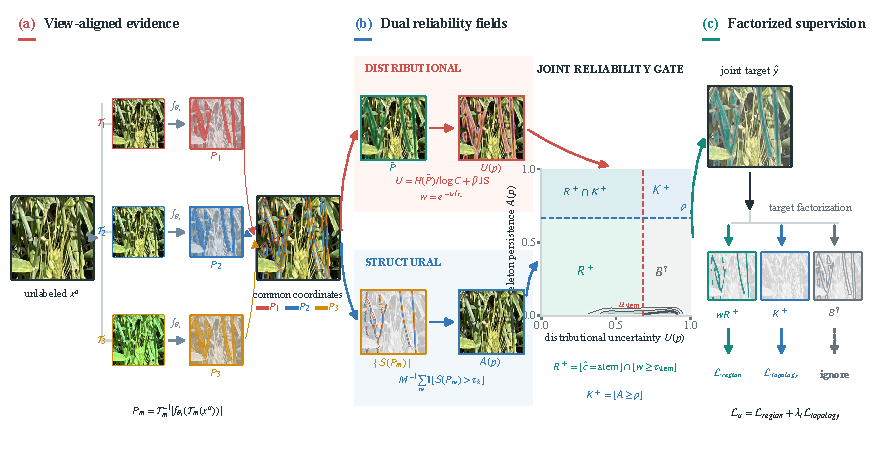
\includegraphics[width=\linewidth]{figures/topology_pseudo_label.pdf}
\caption{\TRPL 的双证据解耦机制。（a）同一幅未标注图像经两个尺度的弱视图和 EMA 教师预测后反变换至公共坐标，形成对齐概率栈 $\{P_m\}$；叠加轮廓揭示了不同视图对茎秆边界宽度的分歧及其共享的轴向结构。（b）分布支路由平均置信度和总变差分歧计算可靠性 $r(p)$，结构支路对齐两个视图的硬预测骨架。单一阈值产生可靠区域，严格骨架交集产生稳定中心线。（c）联合门控在同一空间坐标中分解出加权区域 $rR^+$、稳定中心线 $K^+$ 和忽略边界 $B^{?}$，三者分别连接语义一致性、拓扑一致性和无梯度路径。RGB 来自真实样本；概率场依据其标注几何构造为机制示意，不参与定量结论。}
\label{fig:trpl}
\end{figure}

概率可靠性与结构稳定性的分工在\cref{fig:trpl}中得到直观呈现。记 $\Omega_c=\{p\in R^+\mid\hat y(p)=c\}$，$\mathcal C^+$ 为当前批次中 $\Omega_c$ 非空的类别集合。学生的语义一致性损失采用按类别平均的软 KL：
\begin{equation}
\mathcal L_{\mathrm{semantic}}=
\frac{1}{|\mathcal C^+|}\sum_{c\in\mathcal C^+}
\frac{1}{|\Omega_c|}\sum_{p\in\Omega_c}r(p)
\operatorname{KL}\!\left(\bar P(p)\,\|\,P_s(p)\right),
\label{eq:regionloss}
\end{equation}
其中 $P_s$ 为学生强扰动视图的预测。按类别平均避免背景像素数量支配梯度，软目标则保留教师的类别间不确定性。拓扑监督仅作用于双视图一致的可见中心线：
\begin{equation}
\mathcal L_{\mathrm{topology}}
=-\frac{1}{|K^+|}\sum_{p\in K^+}
\log\max_{q\in\mathcal N_1(p)}P_s^{\mathrm{stem}}(q),
\label{eq:topoloss}
\end{equation}
其中一像素邻域 $\mathcal N_1$ 容忍缩放与反变换造成的离散偏移。最终 $\mathcal L_{\mathrm{TRPL}}=\mathcal L_{\mathrm{semantic}}+\lambda_t\mathcal L_{\mathrm{topology}}$。该设计不对两个可见端点之间执行形态学连线，也不在有标注分支额外叠加损失，因此不会把偶然误连固化或改变监督基线目标。

\subsection{拓扑核心原型记忆}
\label{sec:tcpm}

类别原型为跨域分割提供了紧凑的语义参照。ProDA 根据像素到类别原型的距离修正伪标签并压紧目标域特征 \citep{zhang2021proda}，Pin the Memory 则通过类别记忆和模拟元测试学习未知域中的共享概念 \citep{kim2022pinmemory}。两者启发了本文的原型约束和留一域训练，但直接从完整高置信区域求均值仍不适合小麦器官：叶片边缘、茎秆边缘和二者交叠位置恰好是域风格与分类噪声最强的区域，少量错误像素就可能显著移动像素占比很低的茎秆原型。反过来，若干净核心既用于建库又作为唯一查询，分割头中已经分离的类别质心很容易满足原型分类，损失会退化为近零的自一致性，真正发生域偏移的器官边缘和遮挡邻域反而得不到校正。\TCPM 因而采用非对称证据流：拓扑核心只负责建立稳定锚点，可靠区域中偏离跨域锚点最明显的特征负责接收梯度。

具体地，本文从像素解码器的高分辨率掩码特征中提取归一化表示 $z(p)$，并为样本 $i$ 的类别 $c$ 定义核心像素集合 $\Omega_{i,c}$。茎秆核心由稳定中心线 $K^+$ 及其窄邻域组成；其余类别使用边界收缩后的高置信内部区域。大面积器官可以舍弃少量边界来换取纯净内部特征，茎秆却必须保住窄结构的轴向证据，因此这里不对四个类别使用相同的形态操作。记证据权重 $w(p)$ 在有标注分支取 1、在伪标注分支取 \TRPL 可靠性 $r(p)$。核心在特征分辨率下少于 $n_{\min}$ 个像素时不更新记忆；其余核心先被压缩为带权样本质心
\begin{equation}
\widetilde q_{i,c}=\mathcal N\!\left(
\frac{\sum_{p\in\Omega_{i,c}}w(p)z(p)}
{\sum_{p\in\Omega_{i,c}}w(p)}\right),
\label{eq:corecentroid}
\end{equation}
其中 $\mathcal N(\cdot)$ 表示 $\ell_2$ 归一化。样本质心只用于更新记忆，因而大面积背景不能凭像素数量支配锚点，可靠区域中的混合特征也不会反向污染原型。

有标注核心和伪标注核心分别写入 $q^L_{c,d}$ 与 $q^P_{c,d}$ 两组类别--域记忆：
\begin{equation}
q^s_{c,d}\leftarrow\mathcal N\!\left(
\mu_s q^s_{c,d}+(1-\mu_s)\,
\operatorname{mean}_{i:d_i=d}\widetilde q_{i,c}\right),
\quad s\in\{L,P\}.
\label{eq:domainprototype}
\end{equation}
两组证据不直接混写。伪标注分支仅接收 $w(p)\geq\tau_{\mathrm{mem}}$ 且核心大小不小于 $n_{\min}$ 的样本，并采用更大的 $\mu_P$ 抑制单批伪标签的扰动。对于来自域 $d_i$ 的当前质心，类别参照由其余源域构成：
\begin{equation}
q_c^{s,(-d_i)}=\mathcal N\!\left(
\frac{\sum_{d\neq d_i}a^s_{c,d}q^s_{c,d}}
{\sum_{d\neq d_i}a^s_{c,d}}\right),\qquad
\bar q_c^{(-d_i)}=\mathcal N\!\left(
(1-\eta_t)q_c^{L,(-d_i)}+\eta_t q_c^{P,(-d_i)}\right),
\label{eq:lodoanchor}
\end{equation}
其中 $a^s_{c,d}$ 表示对应记忆是否已经初始化，$0\leq\eta_t\leq\eta_{\max}$。当伪标注参照尚不存在时只使用有标注参照；若不存在可用的有标注参照，则跳过该类别的当前原型项，不让伪标注单独定义语义锚点。该构造对批内每个样本分别排除自身域，而不是在一段迭代中冻结某个固定域；所有满足条件的域仍持续更新，因而不会因为阶段性域冻结形成陈旧原型。

锚点建立后，监督分支以全部有效标注区域作为查询候选，伪标注分支则使用通过 \TRPL 可靠性检验且 $w(p)\geq\tau_q$ 的区域。记样本 $i$、类别 $c$ 的候选集合为 $\mathcal R_{i,c}$，其跨域困难度为
\begin{equation}
h_{i,c}(p)=1-\operatorname{sim}\left(z_i(p),\bar q_c^{(-d_i)}\right),\qquad
\mathcal H_{i,c}=\operatorname{Top}_{\kappa}\{h_{i,c}(p):p\in\mathcal R_{i,c}\},
\label{eq:hardquery}
\end{equation}
其中 $\operatorname{Top}_{\kappa}$ 保留困难度最高的 $\kappa$ 比例。候选过多时先作空间均匀抽样再排序，避免相邻的大面积背景重复占据查询预算。核心像素仍可能进入候选集，但只有偏离留一域锚点的部分会被选中，因此记忆写入和损失读取不再是同一条容易路径。

令 $\mathcal A$ 表示具有正确类别锚点的样本--类别记录集合，$Z_{i,c}=\sum_{p\in\mathcal H_{i,c}}w(p)$。为防止背景等大面积类别支配优化，实现中先在每条样本--类别记录内按置信度归一，再对有效记录等权平均。记 $\mathcal A_{\mathrm{con}}\subseteq\mathcal A$ 为至少存在两个可用类别锚点的记录，$\mathcal C_i^{(-d_i)}$ 为其可用锚点类别集合，则困难查询的原型对比损失为
\begin{equation}
\mathcal L_{\mathrm{con}}=
-\frac{1}{|\mathcal A_{\mathrm{con}}|}
\sum_{(i,c)\in\mathcal A_{\mathrm{con}}}\frac{1}{Z_{i,c}}
\sum_{p\in\mathcal H_{i,c}}w(p)
\log\frac{\exp(\operatorname{sim}(z_i(p),\bar q_c^{(-d_i)})/\tau_p)}
{\sum_{c'\in\mathcal C_i^{(-d_i)}}\exp(\operatorname{sim}(z_i(p),\bar q_{c'}^{(-d_i)})/\tau_p)},
\label{eq:contrastive}
\end{equation}
同类对齐不要求所有域内特征坍缩到同一点，而只惩罚超过容差 $\delta$ 的偏差：
\begin{equation}
\mathcal L_{\mathrm{dom}}=
\frac{1}{|\mathcal A|}\sum_{(i,c)\in\mathcal A}\frac{1}{Z_{i,c}}
\sum_{p\in\mathcal H_{i,c}}w(p)
\left[1-\operatorname{sim}(z_i(p),\bar q_c^{(-d_i)})-\delta\right]_+.
\label{eq:domaincompact}
\end{equation}
对于容易混淆的茎秆与叶片，另设困难负样本项
\begin{equation}
\mathcal L_{\mathrm{hn}}=
\frac{1}{|\mathcal A_{sl}|}\sum_{(i,c)\in\mathcal A_{sl}}\frac{1}{Z_{i,c}}
\sum_{p\in\mathcal H_{i,c}}w(p)
\left[m+\operatorname{sim}(z_i(p),\bar q_{c^-}^{(-d_i)})
-\operatorname{sim}(z_i(p),\bar q_c^{(-d_i)})\right]_+,
\label{eq:hardnegative}
\end{equation}
其中 $\mathcal A_{sl}\subseteq\mathcal A$ 只包含叶片和茎秆锚点均可用的对应记录，$c^-$ 是二者中的另一类别；任一有效集合为空时相应损失记为 0。三项均采用固定查询上限、逐记录类平衡和置信加权，只有困难区域产生原型梯度；核心锚点、容易区域以及容差内的合理域内变化不会被反复压缩。

TCPM 并不随半监督阶段立即全量启用。监督最优权重同步到师生两支后，以 Stage II 的第 0 次迭代为 $t_0$：$[t_0,t_1)$ 只积累有标注记忆，不施加原型损失；$[t_1,t_2)$ 将三项损失由 0 线性增加到设定权重；到 $t_2$ 后才允许满足质量门限的伪标注核心更新第二组记忆，并在随后若干迭代内把 $\eta_t$ 从 0 增至 $\eta_{\max}$。该日程把“教师是否连续更新”和“原型何时参与优化”分开管理，避免中途教师替换与原型启用在同一节点叠加。

\begin{figure}[!htbp]
\centering
%\includegraphics[width=\linewidth]{figures/topology_core_memory.pdf}
\fbox{\parbox{0.94\linewidth}{\centering \vspace{1.05cm}
\placeholder{TCPM 机理图采用“干净核心写入--双记忆聚合--留一域锚点--困难可靠查询”四段式横向流程，并在底部增加独立课程时间轴。第一段在同一幅小麦 RGB、类别掩码和特征网格上同时画两类区域：茎秆核心使用红色骨架窄管，麦穗、叶片和背景核心使用向内收缩的深色实心区域；核心外但通过可靠性检验的器官区域使用浅色半透明覆盖，灰色斜线表示忽略边界。深色核心经置信加权汇聚为样本--类别质心 $\widetilde q_{i,c}$，少于 4 个特征像素时以虚线箭头指向“skip”；浅色区域不得连接记忆写入口。第二段上下排列有标注记忆 $q^L_{c,d}$ 与伪标注记忆 $q^P_{c,d}$，横轴为背景、麦穗、茎秆和叶片，纵轴为 Domain 1 至 Domain 9；实线 EMA 箭头标注 $\mu_L=0.95$，较细虚线箭头标注 $\mu_P=0.995$，伪核心写入口前画 $w\geq0.8$ 门控，两组记忆之间不画直接写入箭头。第三段以灰色横条遮掉当前样本的第 $d_i$ 行，其余域分别聚合为 $q_c^{L,(-d_i)}$ 和 $q_c^{P,(-d_i)}$，再用标有 $(1-\eta_t)$ 与 $\eta_t$ 的两条不同粗细箭头融合为 $\bar q_c^{(-d_i)}$；用两个来自不同当前域的小例子强调排除操作逐样本改变，而所有域仍继续写入。第四段从浅色可靠区域中先做最多 128 点的空间均匀采样，伪标注查询入口标注 $w\geq0.6$，每个点以细线连接正确类别锚点；按余弦距离着色，从蓝色易查询过渡到红色困难查询，仅用粗描边保留距离最高的 25\%。红色查询分别连接原型分类损失、带容差 $\delta$ 的同类对齐损失和叶片--茎秆排序损失；蓝色易查询和容差圆内部画断开的灰色梯度符号，明确其不产生重复压缩。右侧配一组共享坐标轴的前后散点图，展示困难边缘特征向正确锚点移动，而深色核心锚点和合理类内散布基本保持。底部时间轴以 Stage II 为零点，依次标出 0--5k“仅写 $q^L$”、5--15k“损失线性升权”、15k“开放高质量 $q^P$”、25k“$\eta_t=0.2$”；时间轴上方另画教师与学生从同一监督 checkpoint 出发、EMA 连续更新的两条轨迹，禁止出现 20k 硬复制箭头。测试目标域以独立虚线灰框放在全部记忆之外。类别、域、标注来源、写入/读取和有/无梯度箭头必须使用互不混淆且不遮挡组件的图例。}
\vspace{1.05cm}}}
\caption{\TCPM 以拓扑核心建立课程式双记忆，并用逐样本留一域锚点校正可靠区域中的困难查询。}
\label{fig:tcpm}
\end{figure}

如\cref{fig:tcpm}所示，双记忆把人工标注的稳定参照与伪标注带来的外观覆盖分开管理，逐样本留一域只改变当前损失所读取的参照，不阻断任何源域的正常写入。核心--查询非对称性进一步把“哪些特征可信”与“哪些特征需要校正”分开：前者决定锚点，后者决定梯度位置，从而避免容易核心形成近零损失，也避免边缘噪声移动记忆。

\subsection{断裂感知选择性放大}
\label{sec:bazr}

选择性细化并非新的计算范式。PointRend 在不确定点上迭代预测以恢复清晰边界 \citep{kirillov2020pointrend}。Liu 等人的 SparseRefine 用预测熵筛选少量高分辨率像素 \citep{liu2024sparserefine}，HRDA 也说明局部高分辨率与全局上下文需要共同保留 \citep{hoyer2022hrda}。这些方法主要把高熵或边界视为细化依据；对于小麦茎秆，一段预测可以具有较高置信度却在低分辨率下发生断裂，普通叶片边缘又可能具有高熵但并不需要额外计算。项目原方案采用密集多尺度滑窗缓解这一问题 \citep{cao2025detailminority}，代价是所有位置都被重复处理。\BAZR 沿用“把高分辨率计算留给困难位置”的思想，但把路由单位从像素改为窗口，并把结构断裂而非单纯分类不确定性纳入选择标准。

\BAZR 对完整图像执行一次全局推理，得到概率图 $P^g$。为避免在路由阶段再次运行完整多尺度模型，本文在像素解码器的高、低分辨率特征上设置轻量辅助预测头，并在同一次前向过程中得到 $P^{\mathrm{high}}_{\mathrm{aux}}$ 和 $P^{\mathrm{low}}_{\mathrm{aux}}$。

将图像划分为候选窗口 $\{\mathcal W_k\}$。第 $k$ 个窗口的细化优先级为
\begin{equation}
r_k=
a\,\overline U_k
+b\,E_k
+c\,D_k
+d\,\overline P^{g,\mathrm{stem}}_k,
\label{eq:routingscore}
\end{equation}
其中 $\overline U_k$ 为全局预测的平均归一化熵，$E_k$ 为异常骨架端点密度，$D_k$ 为两个辅助预测头在茎秆类别上的平均差异，$\overline P^{g,\mathrm{stem}}_k$ 为平均茎秆概率。$E_k$ 使模型关注可能发生断裂的细长组件，$D_k$ 则反映网络内部不同空间尺度对该区域的判断分歧。

本文使用非极大值抑制去除高度重叠窗口，并选择得分最高的 $K$ 个窗口。每个窗口从原始图像裁剪后放大至网络输入尺寸，复用同一分割器得到局部高分辨率预测 $P_k^z$。局部与全局预测通过轻量门控函数融合：
\begin{equation}
P^{\mathrm{final}}(p)=
g_k(p)P_k^z(p)
+[1-g_k(p)]P^g(p),
\quad p\in\mathcal W_k,
\label{eq:fusion}
\end{equation}
窗口外保持 $P^{\mathrm{final}}=P^g$。门控函数在有标注源域和高可靠伪标签上训练，不使用目标域标签。最终推理仅需 $1+K$ 次分割器前向计算。

\begin{figure*}[!htbp]
\centering
%\includegraphics[width=\linewidth]{figures/selective_zoom.pdf}
\fbox{\parbox{0.94\linewidth}{\centering \vspace{1.0cm}
\placeholder{BAZR 机理图以一张包含细茎、叶片交叠和大面积背景的小麦图像为起点。顶部为单次全局前向，主预测头、高分辨率辅助头和低分辨率辅助头从共享特征同时输出结果。中部四张与原图对齐的热图依次表示归一化熵 $U$、异常骨架端点密度 $E$、两个辅助头的茎秆分歧 $D$ 和全局茎秆概率；相同候选网格覆盖四张热图，四项信号按照 $a$、$b$、$c$、$d$ 加权形成窗口分数 $r_k$。NMS 模块滤除重叠候选并保留带编号的 Top-$K$ 窗口，各窗口从原始分辨率 RGB 中裁剪、放大并送入共享分割器，局部结果经空间门控 $g_k$ 与全局预测融合。右侧局部对照标记了断裂茎秆的连接恢复以及保持不变的正确叶片边界。底部比较两条计算路径：密集多尺度方案以覆盖全图的滑窗产生约 160 次前向，BAZR 由一次全局前向和 $K$ 次局部前向组成；反事实案例分别显示未被选择的高熵普通叶片边界，以及被选中的中等熵异常断茎。}
\vspace{1.0cm}}}
\caption{\BAZR 根据茎秆结构失效风险分配高分辨率计算，而非均匀处理整幅图像。}
\label{fig:bazr}
\end{figure*}

熵与结构风险对计算路由的不同作用在\cref{fig:bazr}中得到对照。只有当窗口得分得到多源证据共同支持时，局部预测才会替换全局结果；门控融合则限制修正范围，避免高分辨率裁剪失去全局上下文后破坏已经正确的区域。

\subsection{训练目标与优化过程}

有标注数据仅使用 Mask2Former 原有的类别、掩码交叉熵和 Dice 损失，记为 $\mathcal L_{\mathrm{sup}}$；这保证监督分支与统一主干基线完全一致。原型学习损失为
\begin{equation}
\mathcal L_{\mathrm{prototype}}
=\mathcal L_{\mathrm{con}}
+\gamma\mathcal L_{\mathrm{dom}}
+\xi\mathcal L_{\mathrm{hn}}.
\end{equation}
局部融合门控的监督记为 $\mathcal L_{\mathrm{route}}$。完整训练目标为
\begin{equation}
\mathcal L=
\mathcal L_{\mathrm{sup}}
+\lambda_u\mathcal L_{\mathrm{TRPL}}
+\lambda_p\mathcal L_{\mathrm{prototype}}
+\lambda_r\mathcal L_{\mathrm{route}}.
\label{eq:total}
\end{equation}

训练由监督预热和半监督联合优化组成。监督预热只使用有标注图像，模型选择后将同一组最优参数同时加载到教师和学生；二者不存在重新初始化的分割头。进入联合优化后，学生同时接收有标注图像与按域均衡采样的无标注图像，教师从第一步起按\cref{eq:ema}连续更新。TCPM 同步清空记忆，但前 5,000 次只写入有标注核心，随后逐步开放困难查询损失和高质量伪标注记忆；逐样本留一域参照随当前样本动态构造，不设置固定域冻结周期。具体权重与训练节点见\cref{sec:implementation}。
